\documentclass{standalone}
\usepackage{../../../../preamble_formulas}

\begin{document}
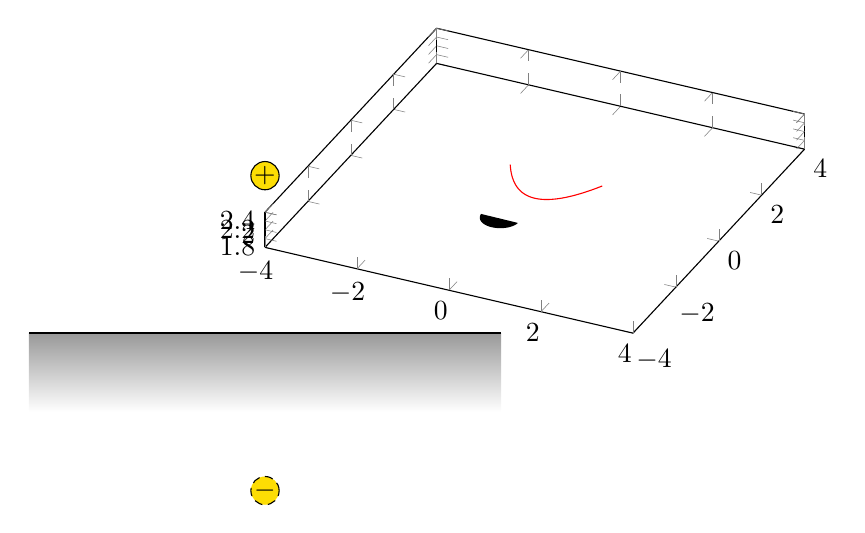
\begin{tikzpicture}
  \def\r{2}
  % surface
  \fill[top color=black!40,bottom color=white] (-3,0) rectangle (3,-1);
  \draw[thick] (-3,0) -- (3,0);

  % % E-field
  % \def\n{8}
  % \def\l{1.8}
  % \foreach \i in{0,...,\n}{
  %     \draw[thin,postaction={decorate},magenta!70!red] (-3,-2*\l/\n*\i+\l) -- (3,-2*\l/\n*\i+\l);
  %   }
  % \node[magenta!70!red] at (2,2){$\vb{E}$};

  % % Ellipse
  % \fill[outer color=green!50!black,inner color=green!10,rotate=45,opacity=0.5] (0,0) ellipse (1.75 and 1);

  % Charges
  \node[circle,draw, fill=yellow!80!orange,inner sep=0] (pos) at (0,\r){$+$};
  \node[circle,draw,densely dashed, fill=yellow!80!orange,inner sep=0] (neg) at (0,-\r){$-$};

  % % Vectors
  % \draw[very thick,-latex] (neg.north east) -- node[anchor=north west]{$\vb{d}$} (pos.south west);
  % \draw[very thick,-latex,blue!90!black] (pos.east) -- node[anchor=south]{$\vb{F}_1$} (2.384,0.884);
  % \draw[very thick,-latex,blue!90!black] (neg.west) -- node[anchor=south]{$\vb{F}_2$} (-2.384,-0.884);
  % \draw[very thick,-latex,blue!90!black,orange!90!black] (0,0) -- node[anchor=south east,pos=0.4]{$\vb{p}$} (0.5,0.5);
  \begin{axis}[axis equal image,domain=-4.05:4.05,,xmin=-4,xmax=4,ymin=-4,ymax=4,samples=40]
    % replace missing field lines at singularities
    \addplot3 [
      domain=-1:1, domain y=-1:1,
      samples=50, samples y=50,
    ] (
    {x*(1/sqrt(x^2+(y-\r)^2)-1/sqrt(x^2+(y+\r)^2))},
    {(y-\r)/sqrt(x^2+(y-\r)^2)-(y+\r)/sqrt(x^2+(y+\r)^2)},
    {2}
    );
    \addplot[red,domain=-1:1](x,x^2);
  \end{axis}
\end{tikzpicture}
\end{document}